\documentclass[tikz]{standalone}
\usetikzlibrary{arrows, chains}

\begin{document}
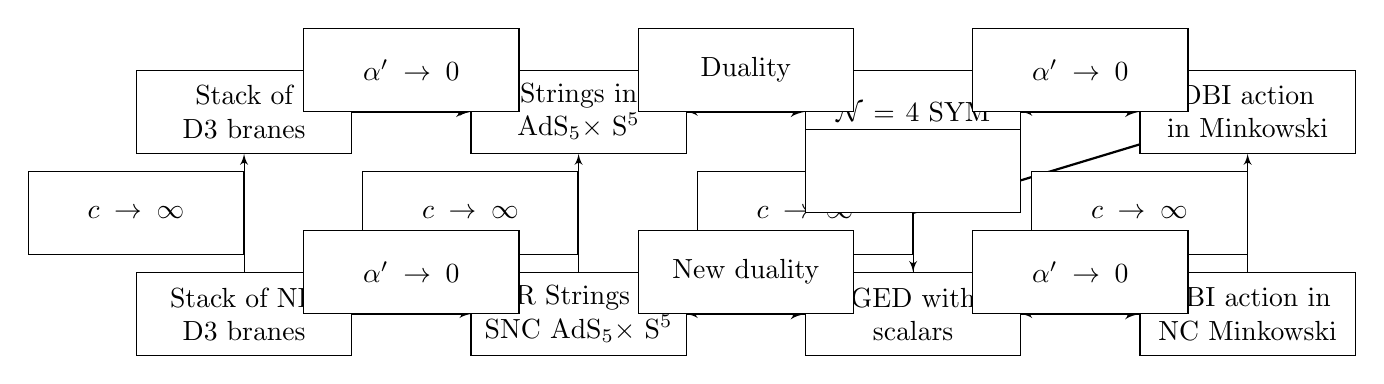
\begin{tikzpicture}[
    start chain = going right,
    node distance = 15mm,
    every node/.style = {draw, fill=white, align=center, minimum height=3em, text width=2.5cm},
    every join/.style = {-latex', thick}
    ]

% First row
\node[on chain] (A1) {Stack of D3 branes};
\node[on chain, join] (A2) {Strings in AdS$_{5} \times$ S$^{5}$};
\node[on chain, join] (A3) {$\mathcal{N} = 4$ SYM};
\node[on chain, join] (A4) {DBI action in Minkowski};

% Second row
\node[below=of A1] (B1) {Stack of NR D3 branes};
\node[on chain, below=of A2, join] (B2) {NR Strings in SNC AdS$_{5} \times$ S$^{5}$};
\node[on chain, join] (B3) {GED with scalars};
\node[on chain, join] (B4) {DBI action in NC Minkowski};

% Arrows for c -> infinity
\draw[latex'-] (A1) -- (B1) node[midway, left] {$c \to \infty$};
\draw[latex'-] (A2) -- (B2) node[midway, left] {$c \to \infty$};
\draw[latex'-] (A3) -- (B3) node[midway, left] {$c \to \infty$};
\draw[latex'-] (A4) -- (B4) node[midway, left] {$c \to \infty$};

% Arrows for alpha' -> 0
\draw[-latex'] (A1) -- (A2) node[midway, above] {$\alpha' \to 0$};
\draw[-latex'] (B1) -- (B2) node[midway, above] {$\alpha' \to 0$};
\draw[-latex'] (A3) -- (A2) node[midway, above, sloped] {Duality};
\draw[-latex'] (B3) -- (B2) node[midway, above, sloped] {New duality};
\draw[-latex'] (A3) -- (B3) node[midway, above] {}; % This was implied for alpha'->0, can be left as is or labeled if needed
\draw[-latex'] (A4) -- (A3) node[midway, above] {$\alpha' \to 0$};
\draw[-latex'] (B4) -- (B3) node[midway, above] {$\alpha' \to 0$};

\end{tikzpicture}
\end{document}